 \subsubsection{UC11 - Visualizzazione delle informazioni utente}
 \begin{figure}[h]
 	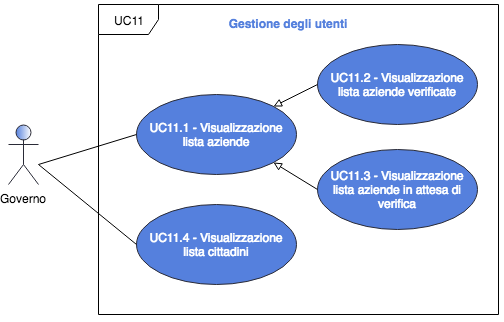
\includegraphics[width=9cm]{res/images/UC11.png}
 	\centering
 	\caption{UC11 - Visualizzazione delle informazioni utente}
 	
 \end{figure}
 \begin{itemize}
 	\item \textbf{Attori Primari}: governo;
 	\item \textbf{Descrizione}: il governo può accedere alle informazioni riguardanti le aziende ed i cittadini che hanno avanzato una richiesta di iscrizione, o che sono già iscritti alla piattaforma. Offre inoltre la possibilità di eseguire delle operazioni su di essi;
 	\item \textbf{Scenario principale}: il governo cerca delle informazioni riguardanti gli utenti della piattaforma e/o esegue delle operazioni su di essi;
 	
 	\item \textbf{Precondizione}: il sistema riconosce che l'utente è autenticato con privilegi governativi e mostra le pagine utili alla ricerca di informazioni sugli utenti;
 	
 	\item \textbf{Postcondizione}: il governo ottiene dal sistema la lista degli utenti dei quali cercava delle informazioni, assieme al set di operazioni che possono essere effettuate su quella tipologia di utente.
 \end{itemize}
 \subsubsection{UC11.1 - Visualizzazione lista aziende}
 \begin{itemize}
 	\item \textbf{Attori Primari}: governo;
 	\item \textbf{Descrizione}: il governo accede ad una lista di aziende, nella quale vengono mostrate tutte le informazioni utili ed operazioni disponibili. In particolare avviene la:
 	\begin{itemize}
 		\item visualizzazione della chiave\glosp Ethereum;
 		\item visualizzazione del nome;
 		\item visualizzazione della partita IVA;
 		\item visualizzazione dell'indirizzo di residenza;
 	\end{itemize}
 	\item \textbf{Scenario principale}: il governo può voler ottenere la lista di tutte le aziende:
 	\begin{enumerate}[label=\alph*.]
 		\item iscritte alla piattaforma con le relative informazioni riguardanti l'IVA [UC11.2];
 		\item che attualmente hanno fatto richiesta di registrazione alla piattaforma, ed eventualmente gestirne la richiesta [UC11.3];
 	\end{enumerate}
	\item \textbf{Specializzazione}:
	\begin{itemize}
	 	\item \textbf{UC11.2}: il governo vuole ottenere le informazioni relative alle aziende che sono già registrate alla piattaforma. In questo caso saranno presenti anche delle informazioni riguardati la situazione IVA delle aziende;
	 	\item \textbf{UC11.3}: il governo vuole ottenere le informazioni relative alle aziende che sono in attesa di essere verificate, per poter poi usufruire della piattaforma. Da questa vista verranno offerte al governo le operazioni di approvazioni/rigetto della richiesta;
	\end{itemize}
 	\item \textbf{Precondizione}: il sistema riconosce che l'utente è autenticato con privilegi governativi ed ha richiesto le informazioni relative alle aziende;
 	\item \textbf{Postcondizione}: il governo ottiene dal sistema la lista delle aziende cercate con le relative operazioni disponibili.
\end{itemize}
\subsubsection{UC11.2 - Visualizzazione lista aziende verificate}
 \begin{itemize}
	\item \textbf{Attori Primari}: governo;
	\item \textbf{Descrizione}: il governo ottiene la lista delle aziende registrate alla piattaforma e già verificate. Per ogni azienda ottiene, oltre alle informazioni di base [UC11.1], lo stato IVA dell'azienda, ovvero può sapere se l'azienda si trova in stato di credito o di debito con lo stato;
	\item \textbf{Scenario principale}: il governo richiede la lista delle aziende registrate e  già verificate;
	\item \textbf{Precondizione}: il sistema riconosce che l'utente è autenticato con privilegi governativi ed ha richiesto di ottenere la lista di tutte aziende già verificate;
	\item \textbf{Postcondizione}: il governo ottiene dal sistema la lista delle aziende registrate e verificate, con associate le operazioni che può effettuare su di esse.
\end{itemize}
\subsubsection{UC11.3 - Visualizzazione lista aziende in attesa di verifica}

\begin{itemize}
	\item \textbf{Attori Primari}: governo;
	\item \textbf{Descrizione}: il governo ottiene la lista delle aziende che sono in attesa di essere verificate per poter poi usufruire della piattaforma. Per ognuna di esse avrà la possibilità di accettare o rifiutare la richiesta;
	\item \textbf{Scenario principale}: il governo richiede la lista delle aziende che sono in attesa di essere verificate;
	\item \textbf{Precondizione}: il sistema riconosce che l'utente è autenticato con privilegi governativi ed ha richiesto di ottenere la lista di tutte le aziende in attesa di verifica;
	\item \textbf{Postcondizione}: il governo ottiene dal sistema la lista delle aziende in attesa di verifica, con associate le operazioni che può effettuare su di esse.
\end{itemize}
\subsubsection{UC11.4 - Visualizzazione lista cittadini}
\begin{itemize}
	\item \textbf{Attori Primari}: governo;
	\item \textbf{Descrizione}: il governo ottiene la lista dei cittadini. Per ognuno di essi può eseguire:
	\begin{itemize}
		\item visualizzazione della chiave\glosp Ethereum;
		\item visualizzazione del nome;
		\item visualizzazione del cognome;
		\item visualizzazione della codice fiscale;
		\item visualizzazione dell'indirizzo di residenza;
	\end{itemize}
	\item \textbf{Scenario principale}: il governo richiede la lista dei cittadini. Per ognuno di essi visualizza alcune informazioni;
	\item \textbf{Precondizione}: il sistema riconosce che l'utente è autenticato con privilegi governativi ed ha richiesto di ottenere la lista di tutti i cittadini;
	\item \textbf{Postcondizione}: il governo ottiene dal sistema la lista dei cittadini, con associate le operazioni che può effettuare su di essi.
\end{itemize}
